\chapter{Testowanie}
\section{Podstawowe testy dialogowe}
\subsection{Powitania}
Jak wspomniano w poprzednim rozdziale, przygotowano zestaw pytań pozwalający na przywitanie się i pożegnanie się przez bota. Przeprowadzono testy sprawdzające, jak reaguje na powitania użytkownika:

\begin{figure}[ht]
	{\centering
		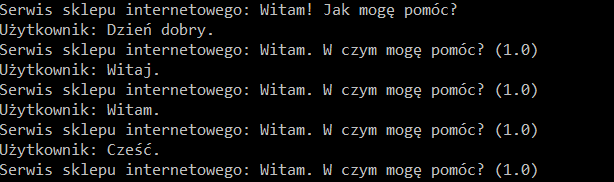
\includegraphics[width=0.9\linewidth]{rys/rys03/1}
	\caption{Reakcja bota na powitania użytkownika.}
	}
	\label{fig:bot4}
\end{figure}

Jak można zaobserwować, pewność odpowiedzi wynosi 100\%. Wynika to z tego, że w bazie wiedzy znajdują się dokładnie te zwroty, których użyto podczas testów.

Kolejnym krokiem było sprawdzenie reakcji na powitania, które zawierają błędy literowe lub zamienioną kolejność wyrazów.

\newpage

\begin{figure}[ht]
	{\centering
		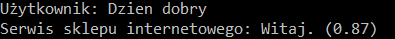
\includegraphics[width=0.9\linewidth]{rys/rys03/2}
	\caption{Reakcja bota na powitanie użytkownika zawierające błąd literowy.}
	}
	\label{fig:bot4}
\end{figure}

Można zaobserwować zmniejszenie pewności odpowiedzi o 13\%.

Kolejnym eksperymentem było sprawdzenie, jak użycie znaków interpunkcyjnych wpływa na pewność odpowiedzi. Wszystkie sekwencje w bazie wiedzy zapisano ze znakami interpunkcyjnymi na końcu zdań oraz pytań. 

\begin{figure}[ht]
	{\centering
		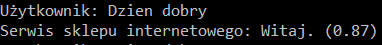
\includegraphics[width=0.9\linewidth]{rys/rys03/3}
	\caption{Powitanie bez znaku interpunkcyjnego na końcu zdania.}
	}
	\label{fig:bot4}
\end{figure}

\begin{figure}[ht]
	{\centering
		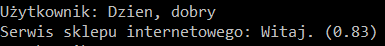
\includegraphics[width=0.9\linewidth]{rys/rys03/4}
	\caption{Powitanie ze znakiem interpunkcyjnym pomiędzy dwoma słowami.}
	}
	\label{fig:bot4}
\end{figure}

Na rysunku 3.3. można zaobserwować obniżenie pewności o 13\%. 
Na rysunku 3.4. widać obniżenie pewności o kolejne 4\% w związku z dodaniem niewystępującego przecinka pomiędzy dwoma wyrazami. 

Wartości te jednak należy uznać za akceptowalne, mając na uwadze, że minimalna pewność odpowiedzi została ustalona na 40\%.

\subsection{Pożegnania}

W bazie wiedzy zawierającej możliwe pożegnania użytkownika zdeklarowano krótkie, w większości składające się z jednego słowa zdania:

\begin{figure}[ht]
	{\centering
		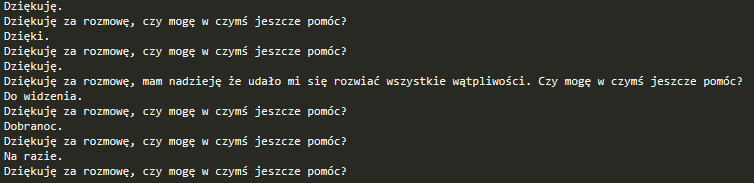
\includegraphics[width=0.9\linewidth]{rys/rys03/6}
	\caption{Baza wiedzy dotycząca pożegnań.}
	}
	\label{fig:bot4}
\end{figure}

Testując interakcję bota w przypadku pożegnania sprawdzono, jak na pewność odpowiedzi wpłynie dodanie dodatkowego słowa do wypopowiedzi użytkownika.

\newpage

\begin{figure}[ht]
	{\centering
		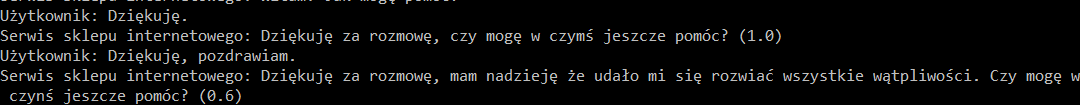
\includegraphics[width=0.9\linewidth]{rys/rys03/5}
	\caption{Pojawienie się dodatkowego słowa w wypowiedzi użytkownika.}
	}
	\label{fig:bot4}
\end{figure}

Na rysunku 3.6. można zaobserwować obniżenie pewności o 40\% w związku z dodaniem jednego słowa do pożegnania.

Kolejnym krokiem było dodanie kolejnego słowa do wypowiedzi użytkownika i sprawdzenie, jak bot poradzi sobie z frazą różniącą się od bazowej o 66\% (3 wyrazy zamiast jednego).

\begin{figure}[ht]
	{\centering
		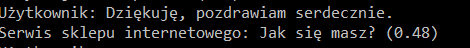
\includegraphics[width=0.9\linewidth]{rys/rys03/7}
	\caption{Pojawienie się dwóch dodatkowych słów w wypowiedzi użytkownika.}
	}
	\label{fig:bot4}
\end{figure}

Zwrócona przez bota nie jest zgodna z oczekiwaną. Współczynnik pewności wynosi 48\% - rozwiązaniem tego problemu mogłoby być m.in.:
\begin{itemize}
	\item
	zwiększenie progu pewności, powyżej którego bot odpowiada na podstawie bazy wiedzy;
	\item
	rozszerzenie bazy wiedzy.
\end{itemize}

\section{Testy zestawów pytań}

Powitania oraz pożegnania to ważna część funkcjonalności bota, jednak nie najważniejsza. Główną funkcjonalność stanowi możliwość pomocy klientowi w podstawych sprawach związanych z zakupami w sklepie internetowym. Kolejnym krokiem było więc przetestowanie wybranych zestawów pytań i odpowiedzi.

\subsection{Pytanie o formę dostawy}

Pierwszym pytaniem, jakie zostało poddane testom, było pytanie o dostępne formy dostawy. W bazie wiedzy zostało ono zapisane w następujący sposób:

\begin{figure}[ht]
	{\centering
		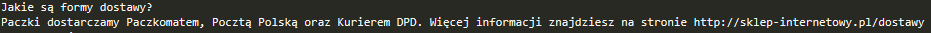
\includegraphics[width=0.9\linewidth]{rys/rys03/8}
	\caption{Pytanie o formy dostawy zapisane w bazie wiedzy.}
	}
	\label{fig:bot4}
\end{figure}

Sprawdzono następujące przypadki:

\begin{itemize}
	\item
	pytanie zgodne w 100\% ze zdefiniowanym w bazie wiedzy.
	\begin{figure}[ht]
	{\centering
		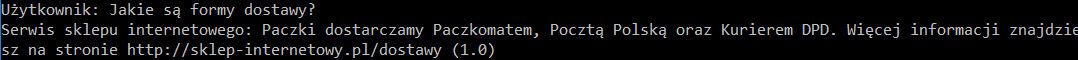
\includegraphics[width=0.9\linewidth]{rys/rys03/9}
	\caption{Odpowiedź bota na pytanie zgodne w 100\% ze zdefiniowanym w bazie wiedzy.}
	}
	\label{fig:bot4}
    \end{figure}
\newpage
	\item
	pytanie bez znaku interpunkcyjnego
		\begin{figure}[ht]
	{\centering
		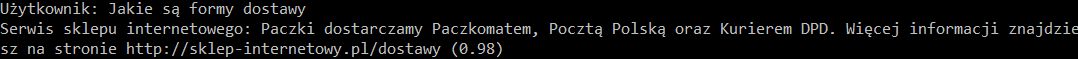
\includegraphics[width=0.9\linewidth]{rys/rys03/10}
	\caption{Odpowiedź bota na pytanie bez znaku interpunkcyjnego.}
	}
	\label{fig:bot4}
    \end{figure}
    
    Warto zwrócić uwagę, że pewność obniżyła się jedynie o 2\%, podczas gdy w przypadku braku znaku interpunkcyjnego dla zdania składającego się z dwóch słów było to 13\%.
	\item
	pytanie zawierające synonim
	\begin{figure}[ht]
	{\centering
		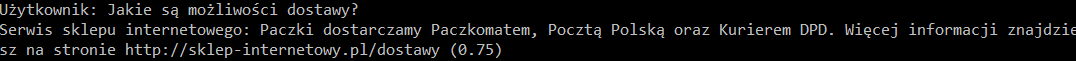
\includegraphics[width=0.9\linewidth]{rys/rys03/11}
	\caption{Odpowiedź bota na pytanie zawierające synonim 'możliwości'.}
	}
	\label{fig:bot4}
    \end{figure}
    
    \begin{figure}[ht]
	{\centering
		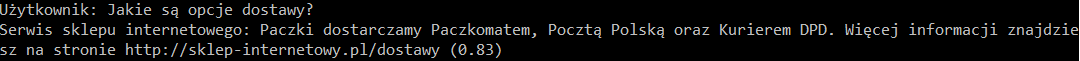
\includegraphics[width=0.9\linewidth]{rys/rys03/12}
	\caption{Odpowiedź bota na pytanie zawierające synonim 'opcje'.}
	}
	\label{fig:bot4}
    \end{figure}
    
    Warto zwrócić uwagę, że pewność boa była inna dla różnych synonimów. Wynika to z liczby znaków poszczególnych synonimów.
	\item
	pytanie zawierające dodatkowe słowo
	
	    \begin{figure}[ht]
	{\centering
		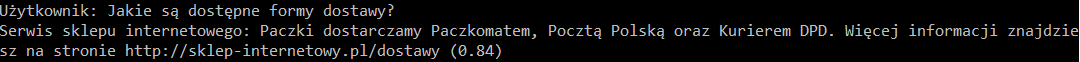
\includegraphics[width=0.9\linewidth]{rys/rys03/13}
	\caption{Odpowiedź bota na pytanie zawierające dodatkowe słowo.}
	}
	\label{fig:bot4}
    \end{figure}
    
    \newpage 
    
	\item
	pytanie zawierające dodatkowe słowo oraz synonim
	
	    \begin{figure}[ht]
	{\centering
		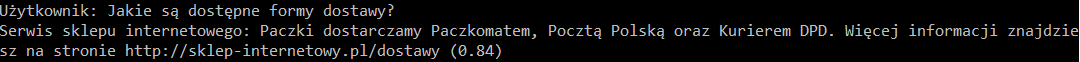
\includegraphics[width=0.9\linewidth]{rys/rys03/13}
	\caption{Odpowiedź bota na pytanie zawierające dodatkowe słowo.}
	}
	\label{fig:bot4}
    \end{figure}
    
\end{itemize}

\subsection{Pytanie o status przesyłki.}

Badany przypadek użycia został w bazie wiedzy zdefiniowany w następujący sposób:

\begin{figure}[ht]
	{\centering
		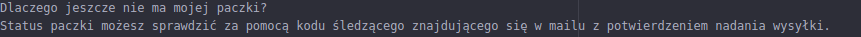
\includegraphics[width=0.9\linewidth]{rys/rys03/15}
	\caption{Definicja pytania w bazie wiedzy}
	}
	\label{fig:bot4}
    \end{figure}

Testom poddano te same sytuacje, co w przypadku poprzedniego pytania. Tym razem jednak badane pytanie zawierało więcej słów.

\begin{itemize}
	\item
	pytanie zgodne w 100\% ze zdefiniowanym w bazie wiedzy.
	\begin{figure}[ht]
	{\centering
		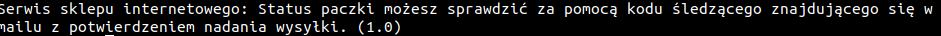
\includegraphics[width=0.9\linewidth]{rys/rys03/16}
	\caption{Odpowiedź bota na pytanie zgodne w 100\% ze zdefiniowanym w bazie wiedzy.}
	}
	\label{fig:bot4}
    \end{figure}

	\item
	pytanie bez znaku interpunkcyjnego
		\begin{figure}[ht]
	{\centering
		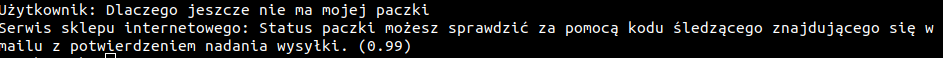
\includegraphics[width=0.9\linewidth]{rys/rys03/17}
	\caption{Odpowiedź bota na pytanie bez znaku interpunkcyjnego.}
	}
	\label{fig:bot4}
    \end{figure}
    
    Po raz kolejny można zaobserwować, że większa liczba słów ma pozytywny wpływ ma pewność odpowiedzi bota w sytuacji pominięcia znaku interpunkcyjnego.
    
    \newpage
    
	\item
	pytanie zawierające synonim
	\begin{figure}[ht]
	{\centering
		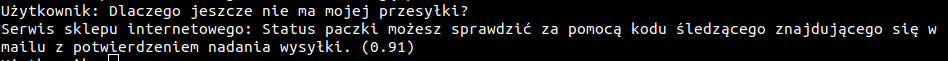
\includegraphics[width=0.9\linewidth]{rys/rys03/18}
	\caption{Odpowiedź bota na pytanie zawierające synonim 'przesyłki'.}
	}
	\label{fig:bot4}
    \end{figure}
    
    
    Pewność bota obniżyła się jedynie o 9\%.
	\item
	pytanie zawierające dodatkowe słowo
	
	    \begin{figure}[ht]
	{\centering
		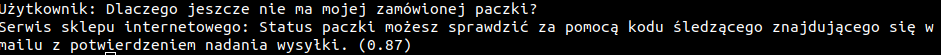
\includegraphics[width=0.9\linewidth]{rys/rys03/19}
	\caption{Odpowiedź bota na pytanie zawierające dodatkowe słowo.}
	}
	\label{fig:bot4}
    \end{figure}
    
    \item
	pytanie zawierające dodatkowe słowo oraz synonim
	
	    \begin{figure}[ht]
	{\centering
		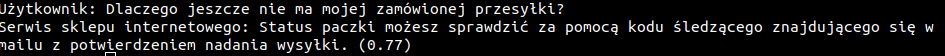
\includegraphics[width=0.9\linewidth]{rys/rys03/20}
	\caption{Odpowiedź bota na pytanie zawierające dodatkowe słowo oraz synonim}
	}
	\label{fig:bot4}
    \end{figure}

\end{itemize}

\newpage
\section{Zwiększanie efektywności bota poprzez zwiększenie bazy wiedzy}

